\chapter{Human Computed Stories in wePorter}
\label{chap:weporter}

[intro: sketch wePorter scenario. youtube: Burning Man 1.7 million, Burning Man 2012 ..., Burning Man this month ...]

[discuss: is wePorter human computation?
is it solving a task that would otherwise be done by computers? By humans? Can it be expected to ever be done by computers? Looking at answers from the questionnaire to the question of why users decided to change their focus, reveal different reasons for their behaviour. A big part of the answers are generic visual or auditory features like the presence of bright colours, video or audio quality and sudden changes in movement of the scenery of camera. These are all aspects of a video that can be computed computationally, some day perhaps even in a realtime online environment. The question whether or not other features such as curiosity or boredom are computable or not is beyond the scope of this thesis, but participants' response hint at the possibility that their interest is at least partially explicable by computable factors.


plot aggregated reasons to change:

cinematography
  camera movement
content based
  action
  trees, boats
visual
  colour
  quality
  changes, movement
audio
  music
Interest, curiosity / boredom
unpleasant
  sound
  visuals
]

\section{Introduction}
This section describes the interaction design of the wePorter system, built to examplify how human computation can be used in tasks like local video part filtering and semi-automated video reconfiguration. The wePorter system runs an interactive webpage that functions as the main source for data acquisition, presentation of results and general proof of concept. In this chapter the system is analysed along the axes of \textit{Purpose}, \textit{Motivation} and \textit{Task}, that were introduced in the analysis of Human Computational systems in chaperter \ref{ch:humancomputation}. Next to these guidelines for analysis, some remarks are made about the specifics in the functioning of the system. Lastly we discuss the implementation of the web application that is central in wePorter.

\section{User Generated Video Content}

[define UGVC]

\url{http://youtube-global.blogspot.co.uk/2009/05/zoinks-20-hours-of-video-uploaded-every_20.html}

\url{http://youtube-global.blogspot.co.uk/2010/03/oops-pow-surprise24-hours-of-video-all.html}

\url{http://youtube-global.blogspot.co.uk/2010/11/great-scott-over-35-hours-of-video.html}
\url{http://youtube-global.blogspot.co.uk/2011/05/thanks-youtube-community-for-two-big.html}
\url{http://youtube-global.blogspot.co.uk/2012/01/holy-nyans-60-hours-per-minute-and-4.html}

\begin{quote}
  Since the dawn of YouTube, we’ve been sharing the hours of video you upload every minute. In 2007 we started at six hours, then in 2010 we were at 24 hours, then 35, then 48, and now...60 hours of video every minute, an increase of more than 25 percent in the last eight months. In other words, you’re uploading one hour of video to YouTube every second. Tick, tock, tick, tock — that’s 4 hours right there!
\end{quote}

These astonishing figures of the amount of video that is uploaded to youtube are nothing short of mind blowing, but will most likely sound dated in a matter of years or even months. Looking at the increase of content uploaded to the video platform in past years, the growth does not seem likely to come to a halt soon [ref table]. All these videos are great for online video junkies, and are increasingly part of the online journalism landscape \cite{Rosenstiel:2012vb}. At the same time, all these videos being put online beg the question which ones of them to watch.

[table of youtube content uploads]

The increasing amounts of content being put online, lead to an information overload and present serious challenges in search and information retrieval tasks [ref]. There is an increased need for ways of aggregation and filtering. Both of these tasks rely heavily on an at least a shallow understanding of what is presented in these media, which, as we've seen in chapter \ref{ch:quest}, is a hard problem to solve via current computational techniques. With so much content being uploaded, how can we find our way in the already enormous ocean of online videos?

\section{The Purpose}

Searching -> IR
With more than an hour of new content per second it is no wonder that youtube has come to be viewed as the go-to for online video, much like ``the digital video repository for the Internet'' that was envisioined by its founders in their first ever blog post [ref http://youtube-global.blogspot.co.uk/2005/07/greetings-everyone-thanks-for-visiting.html]. An important activity on video platforms like youtube is searching and much attention has been given to different methods of multimedia search and indexing [refs]. Youtube's acquisition by Google in 2006 underlines the platform's role as a video search engine. 


\subsection{Different Goals}
Once items have been annotated with tags that reflect the content of a video, these indexes can, along with other meta data of the video, be used for retrieval of videos[ref] in response to textual queries. The effectiveness of such a retrieval task can vary depending on the information that is used in the search algorithm[refs] and the type of content that is searched for \cite{Hollink:2005ei}[more refs]. A third characteristic that determines the effectiveness of a video retrieval system is the goals that users have in their usage of the system. These user goals can vary widely from more to less specific\cite{Davidson:2010tu}. We expand on this latter point, as it forms an important context for the wePorter system.

\subsubsection{Direct Navigation}
First, a user might be drawn to a video platform by a direct link from an external website. Links might be either in the form of actual hyperlinks or playable embedded videos that are followed through to the platform. Navigations via such links form a direct mapping between a user's intention to the desired piece of content. In this case, users have a very specific reason to come and watch. Their desire, at least of knowing the contents of the video, is satisfied after the viewing. YouTube's system engineers call this way of video viewing \emph{direct navigation}\cite{Davidson:2010tu}.

\subsubsection{Search and Goal-oriented browse}
When users have not obtained a direct link to a potentially relevant piece of content, they might still have a specific goal in mind when visiting an online video platform. Reasons to visit might be the wish to see a particular music video or to find an instance of a series by a particular producer. This goal of discovering a rather specific video is referred to as \emph{search and goal-oriented browse}. Provided that the desired piece of content exists and the video platform has an appropriate search function in place, these `narrow queries', will result is a result set of search results from which the user is likely to handpick the sought-after result fairly quickly. Here the user's desired result often lies within a single item of content. Perhaps a few hit and misses are required, but after a couple of clicks the required video is found.

\subsubsection{Unarticulated Want}

[first general unarticulated want, then specifically topically encapsulated browse]

A different scenario emerges altogether when a user approaches a video platform with a more broad and open ended motive. Think for example of someone who wants to know what happened at a large music festival she recently attended, or someone who couldn't make it to a large demonstration and would like to get a sense of the atmosphere. This kind of `broad queries' returns a result set of content in which a users will probably consider many items as a successful retrieval. Furthermore, one could even say that the desired result of a user's query is spread across the multiple pieces of content. By traversing the space of different videos in the result set, users interactively construct the answers to their own queries.

This kind of navigation through a space of related content is common practice on large spaces of linked data[ref]. It has been found that YouTube's related video recommendation functionality, which recommends videos that are related to the video currently being watched, is one of the most important view sources of videos. In fact, traffic received from these recommendations is the main source of views for the majority of videos on YouTube \cite{Zhou:2010ut}. Features derived from users' navigations such as `click-through rate' have been used to improve content-based video recommendation \cite{Yang:2007vb}.

Goal of a person's query in this kind of navigation is no longer defined in a single returnable item of content or even a containable set of items. Rather, the interactive pathway through the a set of interesting bits of content is what represents a user's aim. This broader exploratory goal of finding different parts of relevant content has been termed `unarticulated want'\cite{Davidson:2010tu}.

Interactivity is generally agreed to play an important role in the task of video retrieval, as is reflected by the separate category in the annual TRECVid challenge for interactive video retrieval\cite{Smeaton:2006ww}. Several works have indicated the importance of interactivity in the task of video retrieval to filter through a set of initially returned results \cite{DeRooij:2007ua, Christel:2004wm, DeRooij:2007ua, DeRooij:2008ut}. While most of these systems are aimed at retrieval of clearly specified queries, exemplified by the TRECvid retrieval task, the need for interactive exploration is even more apparent for the broader oriented goal of users engaged in unarticulated want.

\subsection{Serving the Purpose of Unarticulated Want}
The answer to a user's query now lies as much in the journey through the content as in the returned content itself. By traversing from one piece of content to the next, users construct their a sequence of concatenated pieces content. This self-constructed story is an important concept that wePorter capitalises on, as will soon become apparent.

The task at hand of recommending a larger group of interesting videos is radically different compared to the more narrow queries that could be answered by a small set of true positives in an information retrieval task. Besides the spread of the searched for result across different pieces of content, there is a second important difference that lies in the nature of the majority of UGVC.

User-contributed videos commonly consist of raw, unedited footage. In \cite{Rosenstiel:2012vb} Rosentiel and Mitchell report that within the collection they investigated only 39\% of the news-related footage contributed by citizens was edited. It should be noted that this collection contained only the most popular videos per week and that a different distribution will be found in the complete set of news-related videos or all the videos hosted on YouTube. 

Users with broad expectations will not only want to be presented with multiple relevant items from a complete repository, they are also looking for the most interesting parts within these relevant items. This issue is particular to time-based media, and especially relevant for video. Other temporal media, like audio in general and music in particular, have less of a need for segmentation because of  their common usage in multimedia applications. People usually tend to listen to a song entirely and if they which to experience an album in part, constituent songs are already units on their own that can easily be reconfigured. Tag-a-tune is a game with a purpose used to acquire tags for clips of music. Although it could be employed for labelling of smaller audio subclips within songs, the games only aims at global labelling of a sounds\cite{Law:2009vl}.

Because of the raw, unedited nature of the majority of UGVC it is desirable to establish local recommendations that point to `subclips' within a video that are of particular interest. Whereas digital music albums shared online consist of a collection of songs that can each easily be made to stand alone, video currently suffers from a less malleable identity online.  Online videos are currently much like black boxes that can be played, paused, rated, commented on, tagged and shared only in its entirety. What if a piece of raw, unedited UGVC features something spectacular for ten seconds halfway along its timeline, but shows much of the same for the rest of the time? Answering this question will be the first part of the purpose of the wePorter system.

\subsection{Storytelling as Structured Recommendation}

explanation why it is also good to structure the filtered pieces of content into a new configuration.
[TODO]


The ten significant seconds in a two-minute video become a needle in a haystack when an initial set of videos relating to your query includes tens to hundreds of possibly relevant videos with lengths between some tens of seconds and a couple of minutes. The aggregation and reconfiguration of several of these `needles' into a meaningful new whole is another non-trivial task. We present wePorter as a test case for new methods that address both these issues of information overload in video libraries of UGVC. More precisely, wePorter's purpose is two-folded:

From a set of topically related unedited user-generated videos:
\begin{enumerate}
  \item Find localised intervals of interest within each of the source videos
  \item Find a meaningful structure for the reconfiguration of interesing video parts
\end{enumerate}






Idea 1: towards interest based filtering via meaning

Idea 2: skip the semantic gap and directly model human attentional behaviour



many people watching:
Clicking from one video to the next (choosing from a set of related videos)
these inter-video links could be seen as indicators for relatedness and relevance, much like google's page rank algorithm use links across webpages to establish a notion of the most significant site on a particular topic. 

There is an important difference here though. Whereas the links used by Google's search algorithms are embedded in machine readable hyperlinks, the path of clicking on from one video to the next is a characteristic of a person's interaction. 

differences:
	public, readable // private, non readable
	conscious choice // unconcious result of interaction
	Concluding
		can be consciously put in place by several people at large scale // dependent on real `human' traffic.
		

\section{The Motivation}

How to get a group of unrelated people to contribute their efforts to solving the tasks set in our two-folded purpose? This section looks at the reasons people might have to contribute their computational powers to a system with a purpose like wePorter. Looking at the way people engage with online video content on platforms like youtube, we identify patterns in their behaviour that can be matched to a task in a human computation system. This behaviour that is characterised by a more active role in multimedia consumption, can be seen as a larger trend in the development of new media. The end of this section indicates how the motivations of users of the wePorter system can link in with this larger trend. 

\subsection{Information Provision through Online Video}

Since the proliferation of mobile video recording devices, it has become common practice for large-scale (semi-)public events to be covered in UGVC that gets uploaded to the web. While some are critical\cite{Jonsson:2011fh} to the often heralded democratisation and empowerment of people by the new media production and distribution tools, it is clear that the UGVC at places like youtube attracts a lot of traffic from people looking to be informed about recent events. After all UGVC can have its advantages over traditional media when it comes to video news coverage, especially for unexpected events where traditional media do not have the immediacy of user-generated `reports' recorded by coincidental passersby. 

In a recent study as part of the the Pew Research Center’s Project for Excellence in Journalism, the most popular video's from YouTube's `News and Politics' were analysed for a period of 15 months\cite{Rosenstiel:2012vb}. The authors of the study exemplify the power UGVC can have in news provision by showcasing frequently viewed videos detailing scenes from the earthquake and subsequent tsunami that hit Japan in March 2011. The week following the disaster, the 20 most viewed news-related videos on YouTube all related to the catastrophic event and were together viewed more than 96 million times. Most of these videos were recorded by individuals who happened to be in the affected areas when the disaster struck, either uploaded by themselves, or by TV channels who appropriated the content. The study furthermore reports that in the studied period, the most searched term of the month on the YouTube platform as a whole was a news-related event 5 out of 15 months.

While the journalism study above focusses on videos with the `News \& Politics' label, information provision about current events might span a larger set of categories. Someone looking for footage in order to get a sense of the atmosphere at a recent music festival or public demonstration, might very well find relevant videos in categories like `Entertainment', `Travel \& Events' or `Nonprofits \& Activism'. Across all of these categories, we are able to find examples of vast collections of UGVC, uploaded in the period following up newsworthy events.

The wePorter system focusses on these kinds of topically related sets that people are currently exploring interactively by browsing from one video to the next. This way of navigation is an intermediary between the goals of \textit{goal-oriented browse} and \textit{unarticulated want}. The apparently aimless browsing is now encapsulated by the event but users still roam freely within this topicalized set of content. By navigating from video to video, watching some and skipping others, users leave attentional traces that give valuable insight into a user's intentional standpoint.

It is this kind of interactions that are already taking place at a large scale that we like to make use of in the wePorter system. Motivated by the whish to explore informative content, users will instinctively and implicitly contribute their human knowledge to a system that is set up appropriately. This kind of motivation fits the category of `implicity work' as it involves activities that people already enage in for their own reasons\cite{Quinn:2011us}. Considering users' wish to be informed and the interactive way in which they navigate, there is most likely also a factor of enjoyment involved though. We expect though that the more specific motivation of information provision might show to become a valid categorisation for the motivation of people in a HCS as it is a common activity on the web and inherently linked with the hard problem of meaningful interpretation of content.

\section{The Task}

In this section we take a look at how the larger goal of finding intervals of regional interest across time within a single video can be branched out into bite-sized tasks executable by a person in a single interaction. We begin by introducing some conceptual considerations that influenced the interface design. Then a detailed overview of the wePorter web interface is presented. We end with a  section focussing on the implementation of the system.

\subsection{Design Considerations}
Below are included several points that have been instructive in the development of the interactive task central to the wePorter system. Some of these point are system requirements, others are more guiding design principles or thoughts that have been inspiring and formative in the development.

\subsubsection{wePorter is a web interface}
The power of a HCS that relies on data from many interactions is truly unleashed in an online setting, where many people can easily participate and interact. For this goal alone already, wePorter must be a web-based system.
Besides the obvious choice of staying in the realm of the online video content, it makes sense to embed the theoretical explorations of this research in the practicalities of current web technologies. With the ongoing development of technology like HTML5, many new possibilities for a user's web browser are unleashed. The implementation of a research tool concerning online video is a good opportunity for the exploration of the technological possibilities of present day web technologies.

\subsubsection{Hyperlinked Multimedia}
The power of digital content on the internet lies for a great part in its capacity to be hyperlinked. This alleviates the burden of having to host or recompile pieces of media. Instead, files can simply be played and remixed by reference, leaving their respective sources intact and where they are. In the presentation of their digital video repurposing system `Diver', Pea et al. indicate the advantages of using a virtual camera controlled by XML-based files that reference parts of source video instead of rendering new video clips\cite{Pea:2004td}:

\begin{itemize}
  \item ``Virtual video clips eliminate the generation of redundant video files, greatly reducing disk storage requirements.''
  \item ``No rendering time means vastly improved performance. Users can instantly create and play back dynamic path videos without long video-rendering delays.''
\end{itemize}

An implementation of a system where users interact with content that is dynamically reconfigured in real-time will benefit considerably from a hyperlinked functionality, especially when this takes place in an online setting where bandwidth will be limited.

\subsubsection{Localized Interest} % Define `source videos' and `video parts' here?
In order to elicit users' interest in particular parts within a video, we divide each videos in our initial set of topic-related content into smaller parts when presenting them in a user interaction. Slicing up source videos virtually and playing their parts by reference is made possible by a hyperlinked implementation of the video player.

\subsubsection{Interest Elicitation}
The user interaction design should enable means to learn about a user's interest in a video at a particular moment in time. This to the purpose of discovering localised regions of interest within single videos.

% attention -> interest
Considering measures that could indicate how people's interest varies across different videos, an idea that quickly surfaced is that interest might be closely linked to attention. When a piece of content contains something that is interesting to many people, this will most likely result in an increase in views, provided the content is accessible to a variety of people. This simple notion is the idea behind global recommendations that show most popular or `trending' content. Whether the trending item is a video on a sharing platform or a phrase on a microblogging service, when there is a large number of people attending to it, this is a reason to suspect the item to be of interest, even for people who haven't engaged with it yet.

% normally need for personalization
An obvious limitation of these global recommendations is the lack of personalisation. Personalised recommendations are offered because the content that is globally popular may not be related to the topics of my interest. For the purpose wePorter is serving however, focus around a particular topic is already in place and are in the first instance mostly interested at picking out the parts that share a high level of interest globally.

\subsubsection{Recurrent Interaction}
Because of the reliance on data, user's should be able (and encouraged) to engage in the interaction more than once.

\subsubsection{Users Between Consumers and Producers}
Studies reflecting on new media technology and its incorporation in our everyday life are in recent years often speaking of a media convergence, where multimedia content flows dynamically across multiple media platforms and media audiences take an active, participatory role in their search for entertainment experiences. In his book `Convergence Culture', Jenkins writes:

\begin{quote}
  ``This circulation of media content - across different media systems, competing media economies, and national borders - depends heavily on consumers' active participation. I will argue here against the idea that convergence should be understood primarily as a technological process bringing together multiple media function within the same devices. Instead, convergence represents a cultural shit as consumers are encouraged to seek out new information and make connections among dispersed media content. [...] The term \emph{praticipatory culture} contrasts with older notions of passive media spectatorship. Rather htan talking about medie producers and consumers as occupying separate roles, we might now see them as participants who interact with each other according to a new set of rules that none of us fully understands.''
\end{quote}

Surveying the diverse body of research into interactive TV, Cesar and Chorianopoulos propose a new view that considers content editing, content sharing and content control as an alternative to the more hierarchical  `produce-deliver-consume' paradigm associated with traditional media\cite{Cesar:2009fk}. The movement from passive consumers to (inter)active contributors indicates new expectations by users of new media applications. The trend of users' more active engagement in new media technology fits well with the approach of interest defined by users' interaction and our proposal of storytelling as structured recommendation.

\subsubsection{The Death of the Author, the Birth of Collective Creation}
Originally voiced by Roland Barthes, who was contemplating a way of literary writing without the use of a clear narrator. He titled his essay `the death of the author' to signify the lack of presence of an author in written work following this style of writing. In our aim of reconfiguring interesting sub-clips in a new arrangement, the issue of authorship surfaces in a new context. 

Less restrictive forms of digital content licensing, like Creative Commons (CC), mean that it is now possible for content uploaded by its original creator, to be used under specified conditions in a new piece of work by someone else. This kind of licences has been noted to be an important facilitator of research into Human Computation\cite{Law:2009vl}. They make it possible for works not only to be used and remixed by other individuals, but also to be incorporated in algorithmically constructed reconfigurations of user generated content.

Different video platforms are currently offering less-restrictive CC licensing as an integrated part of their services. YouTube currently offers the option of choosing a most basic attribution licence and reports 4 million videos licensed this way \cite{youtubeCC}. The video platform Vimeo focusses on letting video and animation producers share and showcase their original work. The platform has internalized the use of CC from 2010\cite{vimeoTimeline} and many of their users licence their videos such that they can be remixed by others. Figure \ref{fig:vimeoCC} shows that a large part of the licences on the Vimeo platform allow derivatives to be made\cite{vimeoCC}.

\begin{figure}[htbp]
  \centering
    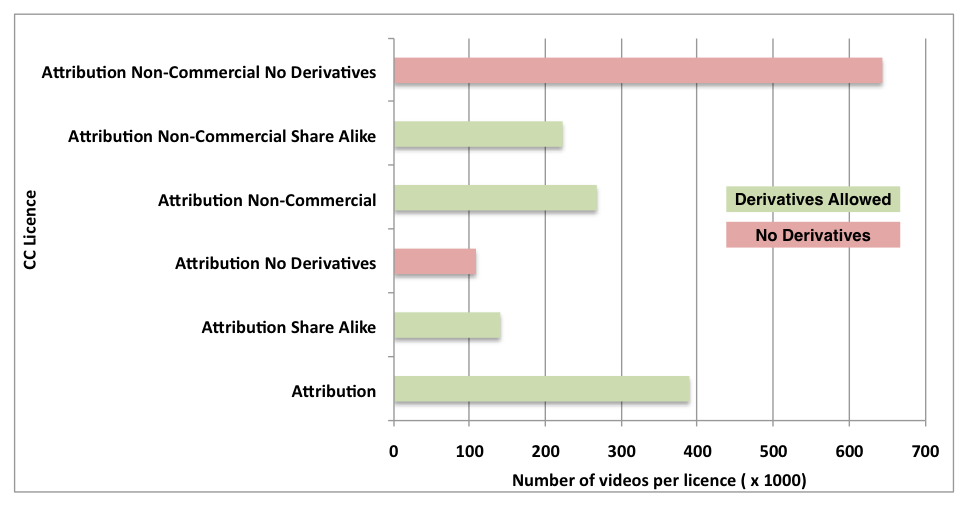
\includegraphics[scale=1]{img/vimeoCC}
  \caption{Number of videos for each of the Creative Commons licences on Vimeo}
  \label{fig:vimeoCC}
\end{figure}

\subsection{The Interface}

This sections describes the user interface that directs participation of wePorter users towards solving the purpose of distinguishing local intervals of interest within videos. After a conceptual overview of the functioning we include a walkthrough to explain precisely how the interaction takes place.

% hypothesis: interest will be reflected in attention
We hypothesise that interesting parts of content will attract a relatively large amount of attention compared to less interesting parts. 

% parallel play; move up to design considerations?
To force a users to make an explicit choice between parts of content for which we would like to elicit their interest, we present two pieces of video playing concurrently and force users to attend to one or the other. In order to get an idea of the variation of interest across a video, \emph{`source videos'} are divided into smaller \emph{`video parts'}, each of which is presented separately in interactions over time. During this `parallel play' of two video parts we capture the amount of time attended to each of the parts and store this for later analysis.

\subsubsection{A Walkthrough}
When a user opens the wePorter web interface he is welcomed by a short introduction to the project and successively guided to further instructions explaining the experiment. Introduction header and instructions are shown in \ref{fig:siteIntro}

\begin{figure}[htbp]
  \centering
    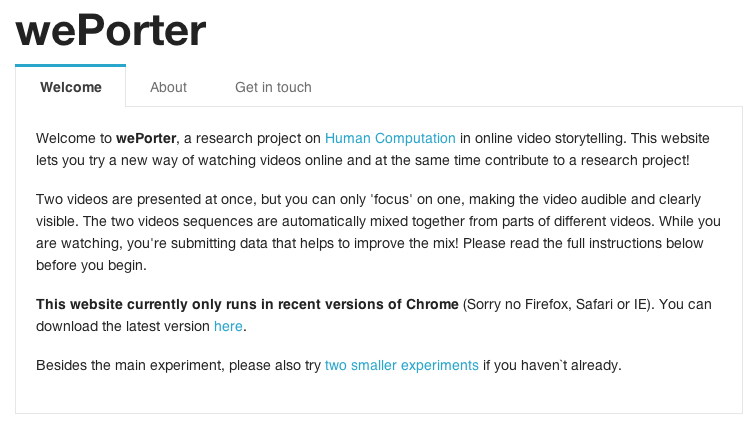
\includegraphics[width=\textwidth]{img/header_noline}
  \caption{wePorter Website Header}
  \label{fig:header}
\end{figure}

\begin{figure}[htbp]
  \centering
    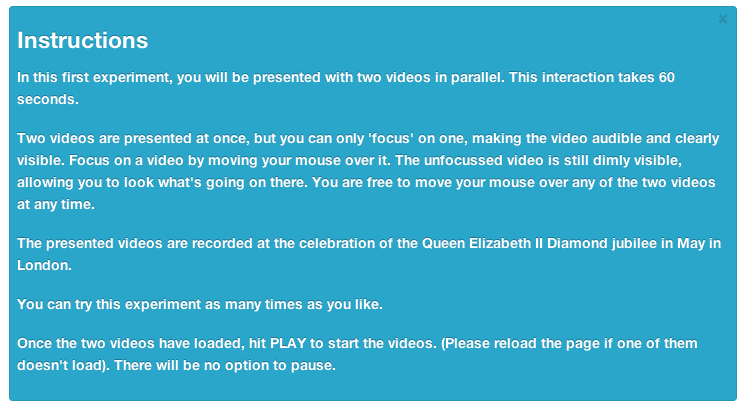
\includegraphics[width=\textwidth]{img/instructions}
  \caption{wePorter Instructions}
  \label{fig:instructions}
\end{figure}


\begin{figure}
  \centering
  \begin{subfigure}[b]{.5\textwidth}
          \centering
          % 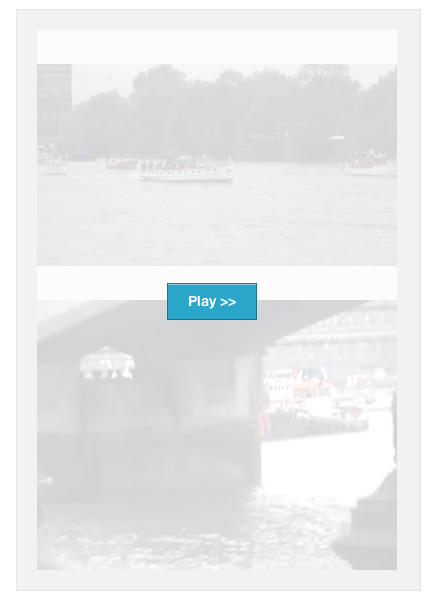
\includegraphics[width=\textwidth]{img/pplay1}
          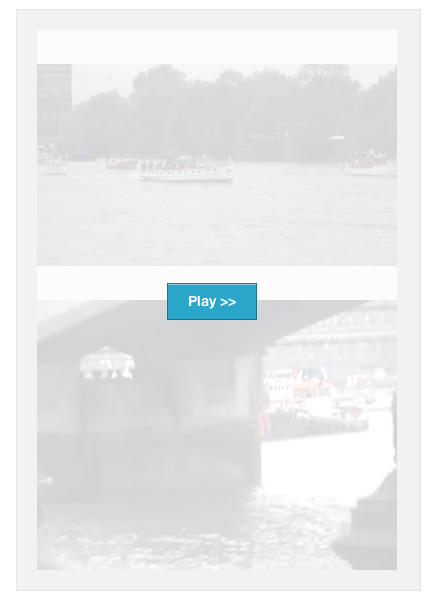
\includegraphics[height=10cm]{img/pplay1}
          \vfil
          \caption{Upon load}
          \label{fig:pplay1}
  \end{subfigure}%
  ~
    %add desired spacing between images, e. g. ~, \quad, \qquad etc. 
    %(or a blank line to force the subfigure onto a new line)
  \begin{subfigure}[b]{.5\textwidth}
          \centering
          % 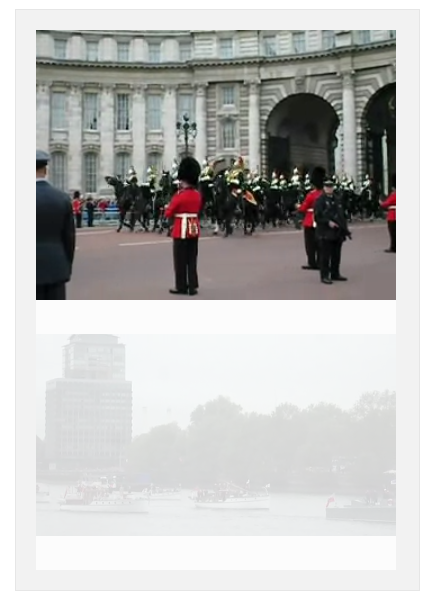
\includegraphics[width=\textwidth]{img/pplay2}
          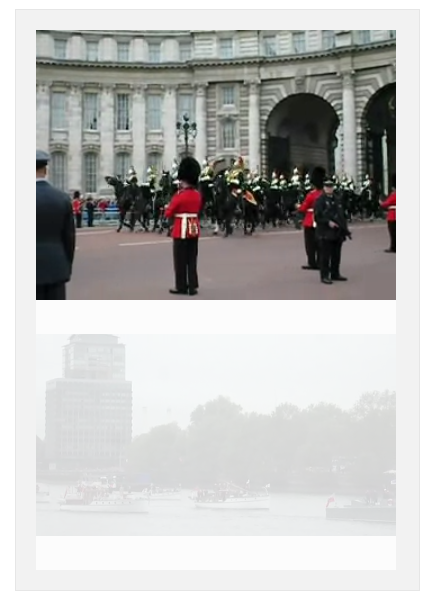
\includegraphics[height=10cm]{img/pplay2}
          \vfil
          \caption{While playing, focus on top video}
          \label{fig:pplay2}
  \end{subfigure}
  \caption{The wePorter parallel play interface}\label{fig:interface}
\end{figure}

% even higher resolution
In its current version the system uses aggregate counts for the time a user focussed on a particular sub-clipd





Parallel player

In the web-based interface two video players are presented at once. When a user initiates an interaction session by hitting play, the two videos start playing. Both videos are now visible to the user, but only one of the audio tracks is played. Users control which player's audio track is being played by moving the mouse cursor over the player they whish to hear. Apart from triggering the audio of a video this way, mouse-over movement also brings focus to a video by displaying it clear, while video out of focus is silent and slightly dimmed.

For every 10th of a second, we record which video a user attends to. Note that we never explicitly ask anyone to point at the video that is most interesting. Users are simply instructed as to how the interface works and then left to explore the video as they like. By recording users' behaviour this way, we achieve a detailed insight as to which of a pair of videos a user has attended to at what time.

Positioning two video's one on top of the other, might inflict a bias for users in their attentional behaviour. It might be the case videos on the top are systematically more attended to than videos displayed below. We've experimented to see whether such positioning bias effects occur and report on this in section \ref{sec:experiments} [*TODO ref].

Sequences of video parts

The video sequences played by the two players consist of distinct parts of videos from a topic-centred video database. This means all content that is aggregated in the interaction is focussed around a single topic, in this example the event of the Queen of England's Diamond Jubilee celebrations in London. The sequences have some other important characteristics:
Sequences are formed out of the same number of video parts (in this example 6)
Video parts in sequences are all of the same duration (in this example 10 seconds)
It follows that all sequences have equal duration (in this example 1 minute).




\subsection{Forced Feedback}
By making data acquisition from interaction an intrinsic part of a human computation system [*need umbrella term], submitting data to the system will become second nature to users and can even take place without the users being aware of it.
	-> curation through interaction


\section{Analysis of the Weporter System}

\subsection{Landscapes of Interest}

The distinction to be made, between interesting intervals on one hand and less striking parts of a video on the other is not likely to be a very strict one. Afterall, an unedited video captures a single strech of space and time, so any event that is of particular interest will unlikely have hard cut-off points in time. Rather, if we see interest as a function of time in a particular video, we would expect a somewhat continuous flowing line with spikes every now and then when an iteresting event occurs. 

Looking at interest at a more global level, aggregating over a large group of users, would perhaps even a more smooth landscape of interest. This kind of data could reveal mountains and valleys that can be used for interest-based segmentation. From the thus segmented parts, the ones with high interest score can be returned as the salient parts within a video.

\subsection{The death of the author}
ref: Barthes - Image music Sound
here: a lack of clear narrator of the written story

in wePorter: the lack of a centralised creator, authoring a work consciously and deliberately.

This new form of creation could at first sight be seen as non-authorship, but is rather a collective authorship. 

Several recent developments now make possible this collective form of authorship:
- the proliferation of tools hhat enable indicidual authorship of multimedia content
- the increased connectivity of these devices, which gives them the capacity to make the created media accessible to others
- the platforms for hosting multimedia (MM) content. This point is strongly related to the previous one. In ther development they form a chicken and egg relaten. Initially it's hard to imagine one withour the other, but once matured, they [influence eachother positively].
- the Methods to link, mix, aggregate and modify content online.

\section{Parallel Play}
A new method for preference elicitation in time-based multimedia content.



and a task is set up such that their interactions are recorded as contributions to solving small instances of a larger problem we have two of the three ingredients of our human computation system in place.

\section{Implementation}
\label{sec:implementation}

% can handle videos of different dimensions

$\underset{x}{\operatorname{argmin}}$

\begin{algorithm}
  \caption{My algorithm}
  \begin{algorithmic}[1]
    \Procedure{Euclid}{$a,b$}\Comment{The g.c.d. of a and b}
      \State $r\gets a\bmod b$
      \While{$r\not=0$}\Comment{We have the answer if r is 0}
        \State $a\gets b$
        \State $b\gets r$
        \State $r\gets a\bmod b$
      \EndWhile\label{euclidendwhile}
      \State \textbf{return} $b$\Comment{The gcd is b}
    \EndProcedure

  \end{algorithmic}
\end{algorithm}

% Pseudo Code generate Sequences Random Shuffled
% # fillSeqs
% (seq1, seq2) <- [],[]
% for i <- 0 to n_parts do
%   # select videoParts with different src than the parts already in sequence
%   selection1 <- []
%   selection2 <- []
%   for all vp in videoParts do:    
%     if vp.src not in selection1:
%       add vp to selection1
%     if vp.src not in selection2:
%       add vp to selection2            
% 
%   # seq1: select videoParts that have minimal count
%   minSelection11 <- []
%   minCount1 <- min(count) from selection1
%   for all vp in selection1:
%     if vp.count == minCount1:
%       add vp to minSelection1
%   selected1 <- pick random from minSelection1
%   add selected1 to seq1
% 
%   # seq2: filter videoParts with different src than selected for seq1
%   selection2V = []
%   for vp in selection2:
%     if vp.src != selected1.src:
%       add vp to selection2V
%   # select videoParts that have minimal count
%   minSelection2 <- []
%   minCount2 <- min(count) from selection2
%   for all vp in selection2:
%     if vp.count == minCount2:
%       add vp to minSelection2
%   selected2 <- pick random from minSelection2
%   add selected2 to seq2
% shuffle in unison(seq1, seq2)

\begin{algorithm}
  \caption{Generate Sequences Random Shuffled}
  \begin{algorithmic}[1]
    \Procedure{Fill Sequences}{}\Comment{The g.c.d. of a and b}
      \State $r\gets a\bmod b$
      \While{$r\not=0$}\Comment{We have the answer if r is 0}
        \State $a\gets b$
        \State $b\gets r$
        \State $r\gets a\bmod b$
      \EndWhile
      \State \textbf{return} $b$\Comment{The gcd is b}
    \EndProcedure

  \end{algorithmic}
\end{algorithm}